\documentclass[12pt,a4paper]{exampaper}
\examname{电子电路基础}
\examsidebarfalse

\begin{document}

\examtitle{东南大学试卷（期中卷）}

\vspace{0.8em}

\begin{center}
  \examfield[3.4cm]{课程名称}{电子电路基础}\hspace{0.4em}%
  \examfield[2.2cm]{课程代码}{}\hspace{0.4em}%
  \examfield[1.8cm]{考试学期}{2022-2023-2}\\[0.4em]
  \examfield[4.4cm]{适用专业}{信息工程}\hspace{0.4em}%
  \examfield[2.0cm]{考试形式}{闭\hspace{0.5em}卷}\hspace{0.4em}%
  \examfield[1.9cm]{考试时长}{120\hspace{0.4em}分钟}
\end{center}

\vspace{0.8em}

\examscoretable[3]

\vspace{0.6em}

\examsection{填空题（本题共 4 小题，每小题 2 分，满分 8 分）}
\begin{examquestions}
  \examquestion 为了保证三极管工作在放大区，要求：发射结\underline{\hspace{1.6cm}} 偏置，集电结\underline{\hspace{1.6cm}} 偏置。
  \examquestion 共射、共集和共基三种基本组态放大电路中，输出电阻最小的是\underline{\hspace{1.6cm}}，输入电阻最小的是\underline{\hspace{1.6cm}}。
  \examquestion N 型半导体中多数载流子是\underline{\hspace{1.6cm}}，P 型半导体中少数载流子是\underline{\hspace{1.6cm}}。
  \examquestion FET 是\underline{\hspace{1.6cm}} 控制电流的器件，只依靠一种载流子导电，因而属于单极型器件。
\end{examquestions}

\vspace{0.6em}

\examsection{单项选择题（本题共 3 小题，每小题 2 分，满分 6 分）}
\begin{examquestions}
  \examquestion 在放大电路的晶体管中，电位最高的一个电极是（　　）。

  A.\ PNP 管的集电极

  B.\ PNP 管的发射极

  C.\ NPN 管的发射极

  D.\ NPN 管的基极
  \examquestion 稳压二极管是一个可逆击穿二极管，稳压时工作在（　　）状态。

  A.\ 正偏 \qquad B.\ 反偏 \qquad C.\ 截止
  \examquestion 为了获得反相电压放大，则应选用（　　）放大电路。

  A.\ 共发射极 \qquad B.\ 共集电极

  C.\ 共基极 \qquad D.\ 共栅极
\end{examquestions}

\vspace{0.6em}

\examsection{计算题（本题共 7 小题，满分 83 分）}
\begin{examquestions}[0pt]
  \examquestion 下图 (a) 为钳位电路，图 (b) 为输入正弦波形。设电容 $C$ 上初始电压为 0，$V_m=15\,\mathrm{V}$，二极管导通电压为 0.7\,$\mathrm{V}$，$R_LC$ 数值是信号周期的 10 倍以上。试画出输出信号波形。

  \begin{center}
  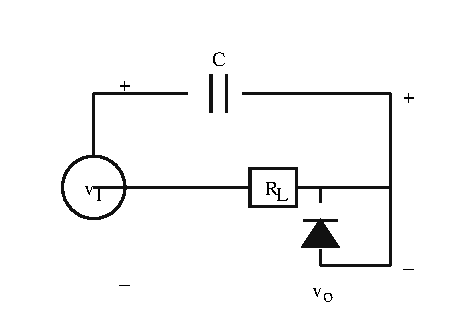
\includegraphics[width=0.46\textwidth]{figures/circuit/c1-clamp-circuit.pdf}\hspace{0.8em}
  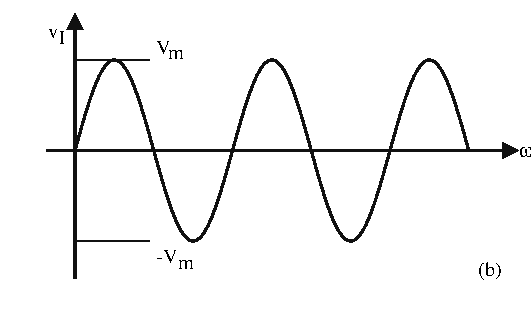
\includegraphics[width=0.50\textwidth]{figures/circuit/c2-clamp-wave.pdf}\\
  \footnotesize 图 1
  \end{center}
  \examanswerspace{7cm}
  \examquestion (1) 分析下图 (a) 所示电路的工作原理，试写出输出信号 $V_O$ 的逻辑表达式；

(2) 图 (b) 中 $V_A$、$V_B$、$V_C$ 为某一电路的输入波形，$V_O$ 为其输出波形。请分析并写出 $V_O$ 与 $V_A$、$V_B$、$V_C$ 的关系式，并设计 CMOS 逻辑门电路实现之，画出设计的逻辑门电路。

  \begin{center}
  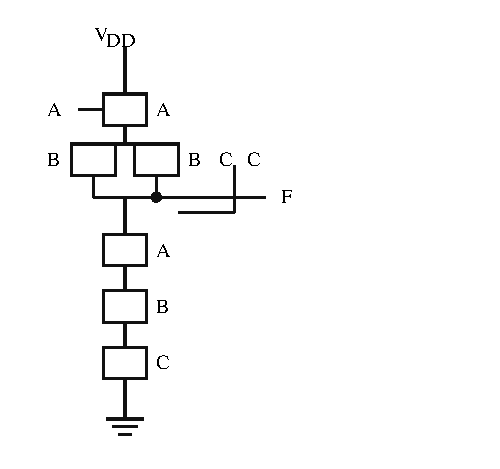
\includegraphics[width=0.40\textwidth]{figures/circuit/c8-cmos-gate.pdf}\hspace{1.2em}
  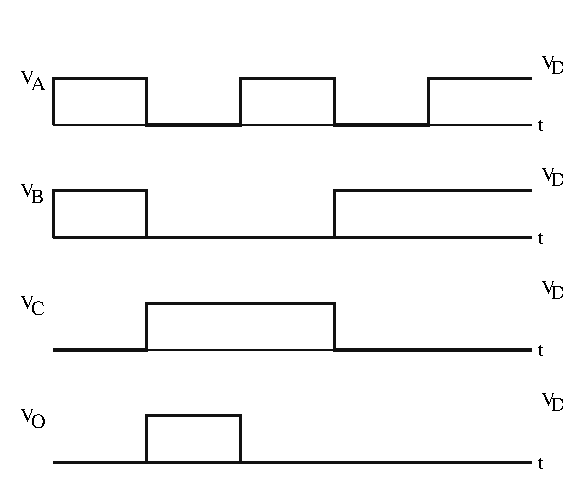
\includegraphics[width=0.50\textwidth]{figures/circuit/c9-gate-wave.pdf}\\
  \footnotesize 图 2
  \end{center}
  \examanswerspace{7cm}
  \examquestion 下图所示为稳压电路，稳压管 $D_1$、$D_2$ 的稳定电压分别是 6\,$\mathrm{V}$ 和 8\,$\mathrm{V}$，导通电压 0.7\,$\mathrm{V}$。试求输出端电压 $V_o$。

  \begin{center}
  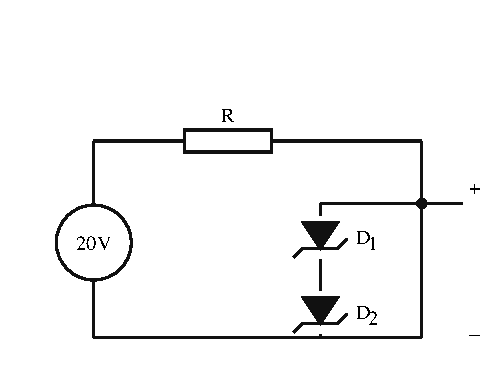
\includegraphics[width=0.50\textwidth]{figures/circuit/c3-zener.pdf}\\
  \footnotesize 图 3
  \end{center}
  \examanswerspace{7cm}
  \examquestion 如图所示，已知 $V_{DD}=10\,\mathrm{V}$，$v_I=(3+0.02\sin\omega t)\,\mathrm{V}$，$\dfrac{1}{2}\mu_n C_{ox}\dfrac{W}{L}=\dfrac{1}{2}\mu_p C_{ox}\dfrac{W}{L}=50\,\mu\mathrm{A}/\mathrm{V}^2$；$T_2$ 管 $V_{GS(th)}$ 绝对值为 2\,$\mathrm{V}$，$T_1$ 管 $V_{GS(th)}$ 绝对值为 1\,$\mathrm{V}$，两管 $V_A$ 绝对值为 100\,$\mathrm{V}$。

(1) 求晶体管 $T_1$、$T_2$ 漏极的直流电流 $I_{D1}$；

(2) 指出 $T_1$ 和 $T_2$ 管的作用；

(3) 画出该电路的小信号等效电路；

(4) 写出该电路的电压增益表达式 $A_v$ 及计算结果；

(5) 求出 $v_o$ 点的瞬时表达式。

  \begin{center}
  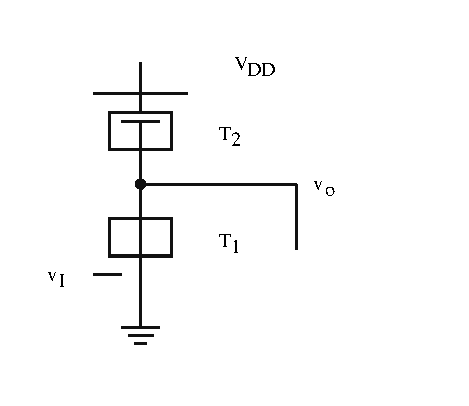
\includegraphics[width=0.38\textwidth]{figures/circuit/c4-cmos-amp.pdf}\\
  \footnotesize 图 4
  \end{center}
  \examanswerspace{7cm}
  \examquestion 下图为两级放大器的交流通路。

(1) 请说明每级放大器的组态；

(2) 写出放大器的增益 $A_v$、源增益 $A_{vs}$ 和输入电阻 $R_i$ 的表达式；

(3) 若信号源电阻 $R_s$ 较大，为了提高源增益 $A_{vs}$，可以在放大器输入端插入一级什么组态的放大器？请简要说明理由。

  \begin{center}
  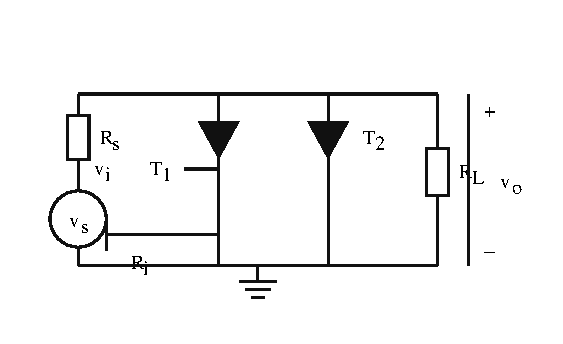
\includegraphics[width=0.68\textwidth]{figures/circuit/c5-multistage.pdf}\\
  \footnotesize 图 5
  \end{center}
  \examanswerspace{7cm}
  \examquestion 下图所示为带恒流源的差分放大电路，设各管参数相同，$V_{BE}=0.7\,\mathrm{V}$，$\beta$ 足够大。试求电路的静态工作点（提示：先计算参考支路电流 $I_{CQ3}$，再计算 $I_{CQ1}$、$I_{CQ2}$）。

  \begin{center}
  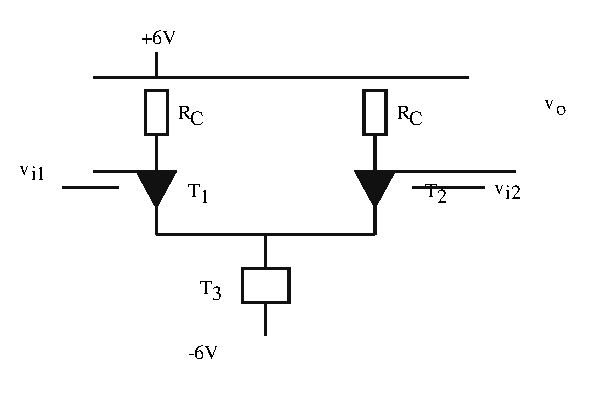
\includegraphics[width=0.64\textwidth]{figures/circuit/c6-diff-amp.pdf}\\
  \footnotesize 图 6
  \end{center}
  \examanswerspace{7cm}
  \examquestion 下图所示为分压式偏置共射放大电路。

(1) 画出直流通路，求静态工作点 $I_{CQ}$、$V_{CEQ}$；

(2) 画出交流通路及微变等效电路；

(3) 求电压增益 $A_v$、输入电阻 $R_i$ 和输出电阻 $R_o$。

  \begin{center}
  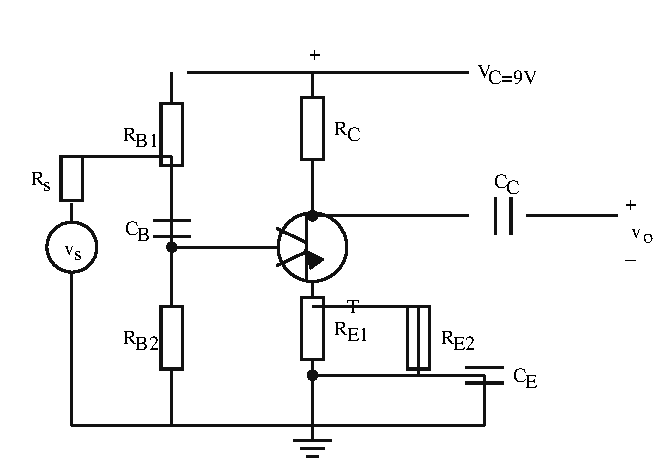
\includegraphics[width=0.74\textwidth]{figures/circuit/c7-ce-amp.pdf}\\
  \footnotesize 图 7
  \end{center}
  \examanswerspace{7cm}
\end{examquestions}

\end{document}
